\label{materials_and_methods}

\subsection{Kiến trúc hệ thống RFAR đề xuất}

\subsubsection{Tổng quan hệ thống}

Hình~\ref{fig:system} minh họa kiến trúc tổng thể và luồng hoạt động của hệ thống RFAR đề xuất. Hệ thống được thiết kế nhằm hỗ trợ trung tâm chỉ huy theo dõi trạng thái hoạt động của từng thành viên đội cứu hộ theo thời gian thực. Mỗi lính cứu hỏa được trang bị một thiết bị đeo nhỏ gọn gắn tại vùng thắt lưng, có khả năng nhận dạng và truyền dữ liệu hoạt động thời gian thực đến thiết bị trung tâm do chỉ huy kiểm soát. Thiết bị trung tâm hiển thị trực quan trạng thái hoạt động của các thành viên, hỗ trợ ra quyết định kịp thời trong tình huống khẩn cấp.

\begin{figure}[!htb]
    \centering
    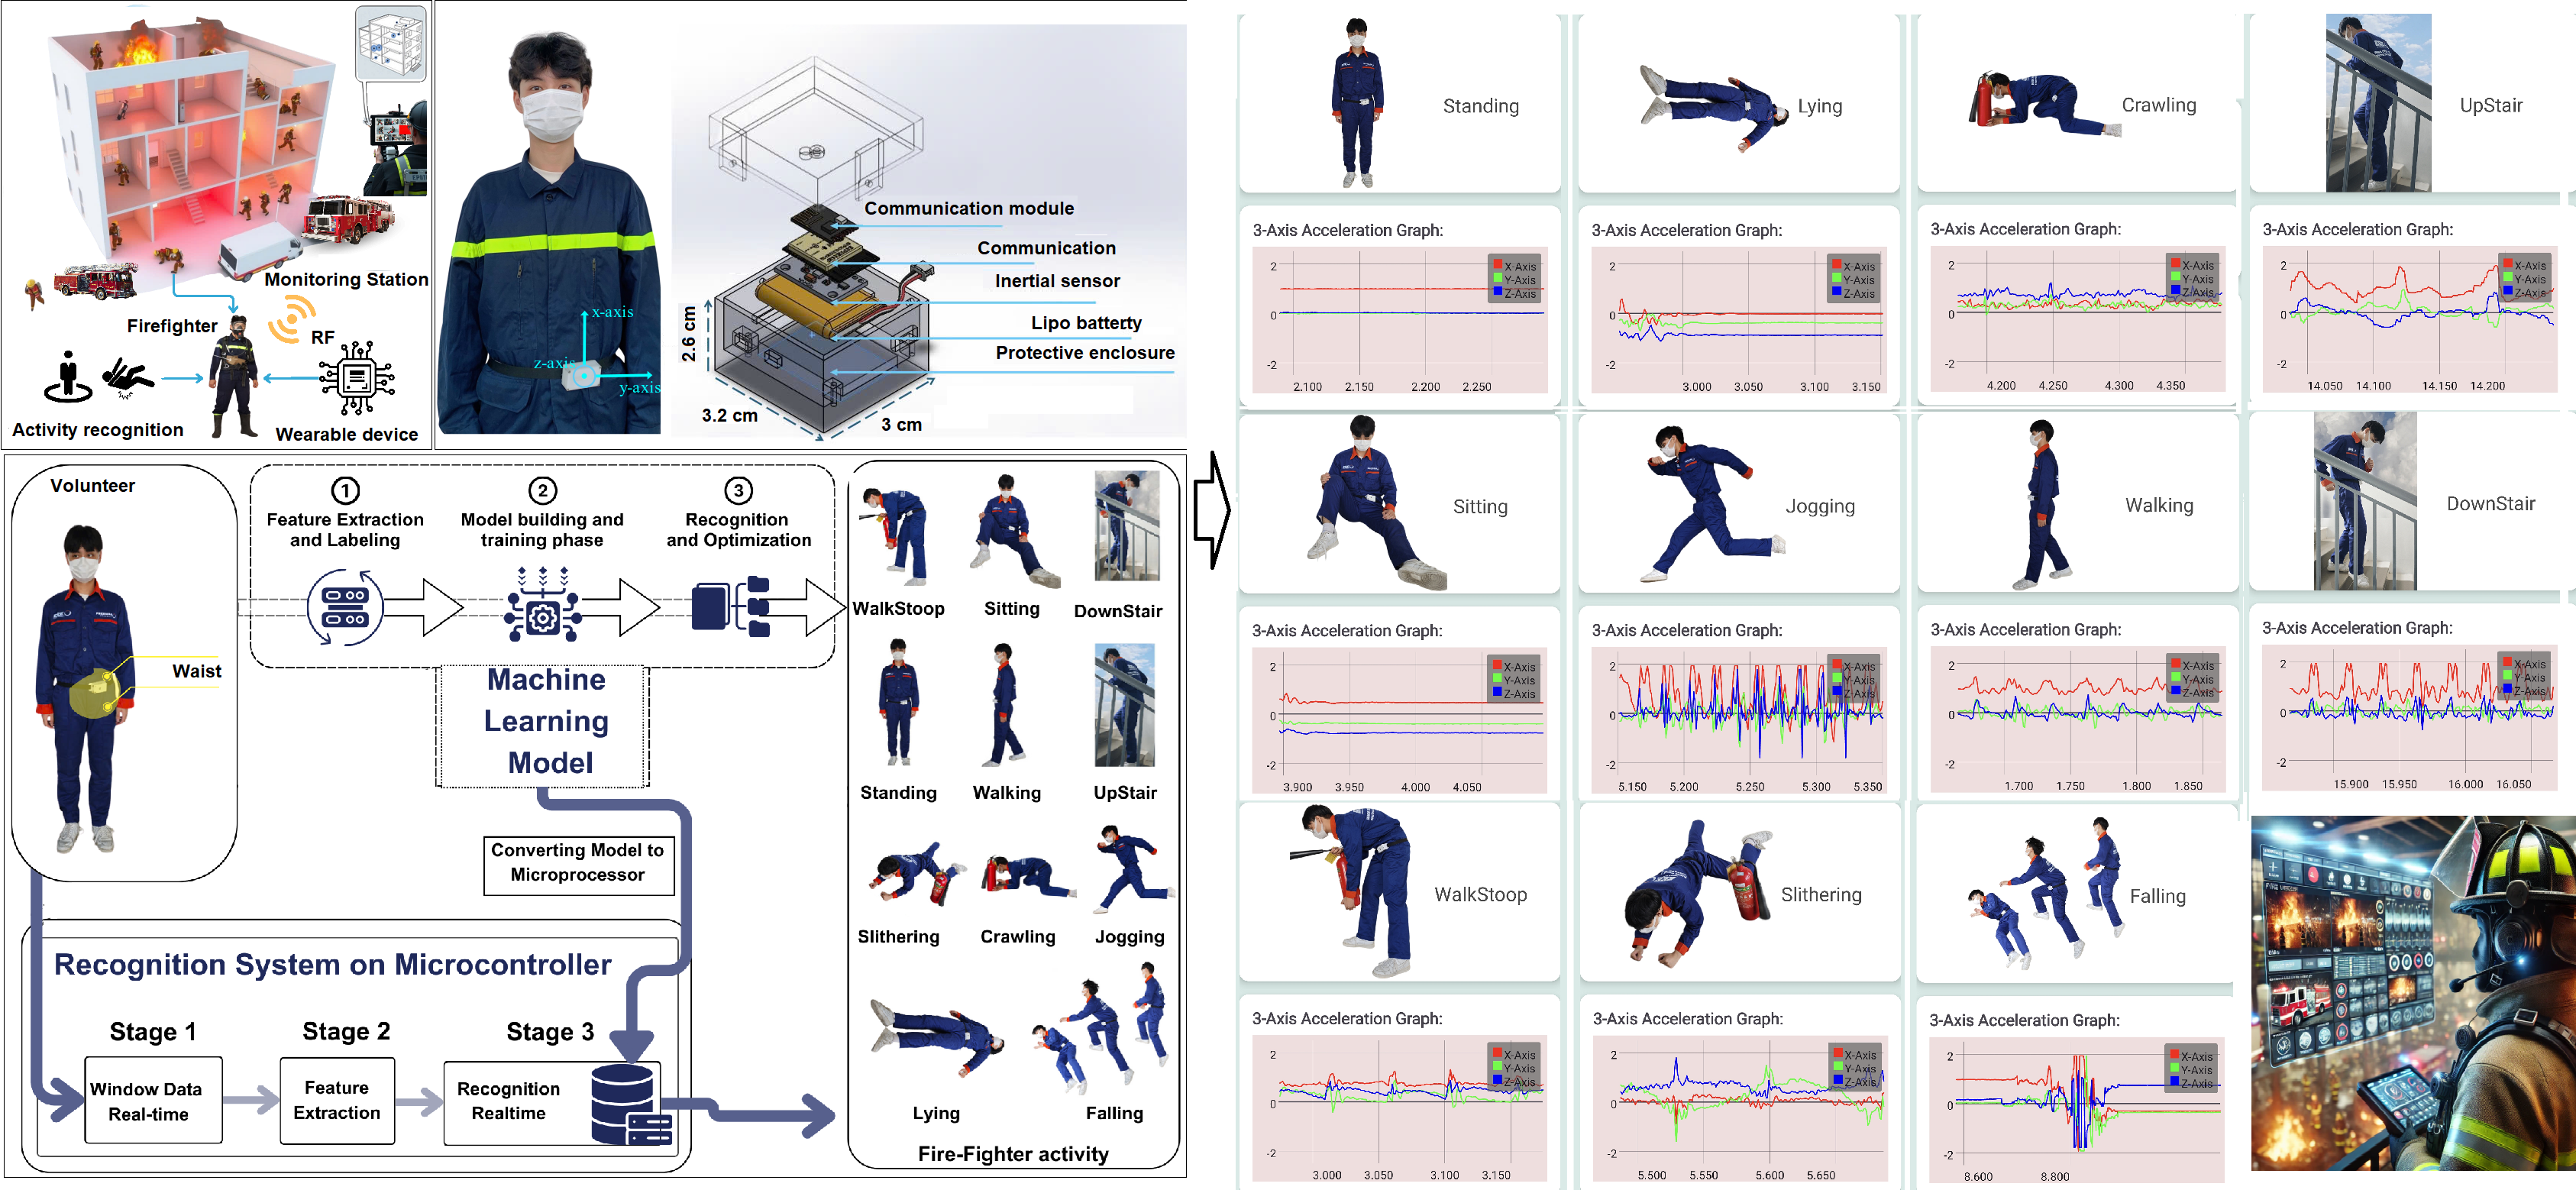
\includegraphics[width=1\linewidth]{Figure/FirefighterSystemfull.png}
    \caption{Kiến trúc tổng thể hệ thống RFAR nhận dạng hoạt động lính cứu hỏa thông qua thiết bị đeo tại thắt lưng, giao tiếp với màn hình chỉ huy qua sóng vô tuyến}
    \label{fig:system}
\end{figure}

\subsubsection{Cấu hình phần cứng}

Cấu hình chi tiết của hệ thống được trình bày trong Bảng~\ref{tab:hardware}. Thiết bị đeo bao gồm cảm biến gia tốc kế ADXL345 ba trục và vi điều khiển ESP32 với 520~KB RAM, 448~KB ROM và 4~MB Flash. Module truyền thông hoạt động ở tần số 433~MHz, đảm bảo khoảng cách truyền tải lên đến 8000~m với tốc độ 2,4~Kbps. Nguồn điện được cung cấp bởi pin Li-ion 2000~mAh, đảm bảo khả năng hoạt động liên tục trên 24~giờ. Toàn bộ thiết bị có trọng lượng dưới 200~g, phù hợp để gắn lên trang phục bảo hộ của lính cứu hỏa.

\begin{table}[!htb]
    \caption{Cấu hình phần cứng và nền tảng thực nghiệm}
    \label{tab:hardware}
    \centering
    \footnotesize
    \renewcommand{\arraystretch}{1.2}
    \resizebox{\linewidth}{!}{
    \begin{tabular}{
        >{\centering\arraybackslash}m{0.15\linewidth}
        >{\arraybackslash}m{0.22\linewidth}
        >{\arraybackslash}m{0.58\linewidth}}
    \hline\hline
    \rowcolor{gray!20}\textbf{Module} & \textbf{Linh kiện} & \textbf{Thông số kỹ thuật} \\
    \hline\hline
    \multirow{5}{*}{\makecell{Thiết bị\\đeo}} & ADXL345 & Gia tốc kế 3 trục kỹ thuật số \\
    & ESP32 & 520~KB RAM, 448~KB ROM, 4~MB Flash \\
    & Thẻ Micro SD & 2~GB \\
    & Truyền thông & 433~MHz; 8000~m; 2,4~Kbps \\
    & Pin & Li-ion, 2000~mAh \\
    \hline
    \multirow{3}{*}{\makecell{Thiết bị\\trung tâm}} & Truyền thông & 433~MHz; 8000~m; 2,4~Kbps \\
    & ESP32 & 520~KB RAM, 448~KB ROM, 4~MB Flash \\
    & Nguồn điện & Bộ chuyển đổi 12~VDC--2A \\
    \hline
    \multirow{5}{*}{Máy chủ} & Chipset & Intel Xeon Silver 4310; 2,1~GHz \\
    & RAM & 16~GB RDIMM \\
    & Ổ cứng & 2~TB IDD NLSAS \\
    & Phần mềm & Visual Studio Code \\
    & Giao thức & MQTT \\
    \hline\hline
    \end{tabular}}
\end{table}

Hệ thống có khả năng nhận dạng mười một hoạt động bao gồm: đi bộ (WA), đứng (ST), nằm (LY), ngồi (SI), chạy bộ (JO), đi khom (WS), bò tay-gối (CR), trườn sát đất (SL), ngã (FA), xuống cầu thang (DS) và lên cầu thang (US). Hệ thống hoạt động theo ba giai đoạn tuần tự: thu thập dữ liệu thời gian thực qua cửa sổ trượt, trích xuất đặc trưng và nhận dạng hoạt động.

\subsection{Xây dựng cơ sở dữ liệu}

\subsubsection{Tập dữ liệu riêng}

Tập dữ liệu lính cứu hỏa được thu thập từ nhóm 20 tình nguyện viên nam trong tình trạng sức khỏe tốt, có độ tuổi từ 22 đến 35, chiều cao từ 1,6 đến 1,8~m và cân nặng từ 60 đến 80~kg. Các tình nguyện viên được tuyển chọn từ Trường Đại học Phenikaa và Trường Đại học Phòng cháy Chữa cháy, không có tình nguyện viên nữ tham gia nhằm đảm bảo đồng nhất về đặc điểm thể chất phù hợp với đối tượng nghiên cứu là lính cứu hỏa nam. Dữ liệu được thu thập tại tần số lấy mẫu 100~Hz, ghi lại giá trị gia tốc ba trục theo đơn vị $g$ ($g = 9{,}8$~m/s$^2$), trong quá trình diễn tập cứu nạn thực tế.

\begin{table}[!htb]
    \caption{Mô tả các hoạt động lính cứu hỏa trong tập dữ liệu riêng}
    \label{tab:activity}
    \centering
    \footnotesize
    \renewcommand{\arraystretch}{1.2}
    \resizebox{\linewidth}{!}{
    \begin{tabular}{>{\centering\arraybackslash}m{0.08\linewidth}m{0.70\linewidth}m{0.12\linewidth}}
    \hline\hline
    \rowcolor{gray!20}\textbf{HĐ} & \textbf{Mô tả} & \textbf{Mẫu} \\
    \hline\hline
    WA & Di chuyển thẳng đứng, duy trì ít nhất một bàn chân tiếp xúc mặt đất & 123.932 \\
    \hline
    ST & Duy trì tư thế thẳng đứng không di chuyển & 56.016 \\
    \hline
    LY & Đặt cơ thể trên mặt phẳng, lưng tiếp xúc mặt đất & 82.516 \\
    \hline
    SI & Tư thế nghỉ với mông và bàn chân tiếp xúc mặt đất & 63.013 \\
    \hline
    JO & Trạng thái di chuyển nhanh, không quá một bàn chân tiếp xúc mặt đất cùng lúc & 90.783 \\
    \hline
    WS & Đi bộ chậm trong tư thế gập hoặc khom lưng & 83.242 \\
    \hline
    CR & Di chuyển về phía trước bằng tay và gối, thân trên nâng nhẹ khỏi mặt đất & 82.669 \\
    \hline
    SL & Di chuyển sát đất bằng tay và gối, cơ thể song song với mặt đất & 90.340 \\
    \hline
    FA & Mất thăng bằng đột ngột dẫn đến tiếp xúc với mặt đất & 129.815 \\
    \hline
    DS & Xuống cầu thang bằng bộ với tốc độ vừa phải & 151.448 \\
    \hline
    US & Lên cầu thang bằng bộ với tốc độ vừa phải & 157.882 \\
    \hline\hline
    \end{tabular}}
    \footnotesize \textit{Chú thích: HĐ = Hoạt động}
\end{table}

Bảng~\ref{tab:activity} trình bày mô tả chi tiết và số lượng mẫu của từng hoạt động. Mỗi hoạt động được thực hiện liên tục ít nhất ba phút, ngoại trừ hoạt động ngã (FA) được thực hiện trong khoảng 3--5 giây. Dữ liệu được lưu trữ trên thẻ nhớ microSD gắn tại thiết bị đeo ở vùng thắt lưng. Tổng thời gian thu thập dữ liệu là 371~phút với tổng kích thước dữ liệu vượt quá 100~MB. Tập dữ liệu được phân chia theo tỉ lệ 60/40 cho tập huấn luyện và kiểm tra.

\subsubsection{Các tập dữ liệu công khai}

Để đánh giá tính khái quát của phương pháp, nghiên cứu sử dụng thêm ba tập dữ liệu công khai có chứa các hoạt động tương đồng:

\begin{itemize}
    \item \textbf{MobiFall} \cite{MobiFall2015}: Bao gồm bốn loại ngã và chín hoạt động sinh hoạt hàng ngày, được thu thập bằng điện thoại thông minh đặt trong túi.
    \item \textbf{SFDLA} \cite{SFDLAdataset2016}: Tập dữ liệu phát hiện ngã và hoạt động dựa trên cảm biến đặt cố định tại thắt lưng.
    \item \textbf{UniMiB-SHAR} \cite{UniMiB_SHAR_2017}: Bao gồm 17 hoạt động từ điện thoại thông minh đặt trong túi trước với hướng cảm biến thay đổi giữa các phiên.
\end{itemize}

Nghiên cứu này áp dụng cách tiếp cận mới, coi ngã là một hành vi cần nhận dạng thay vì coi đó là sự kiện tách biệt, tạo cơ sở so sánh khách quan với các nghiên cứu trước đây về phát hiện ngã và nhận dạng hoạt động.

\subsection{Quy trình xử lý dữ liệu}

\subsubsection{Giảm tần số lấy mẫu}

Để tối ưu hiệu quả xử lý, tần số lấy mẫu được giảm từ 100~Hz xuống 50~Hz thông qua bộ lọc trung bình trượt. Với mỗi trục $k \in \{x, y, z\}$, tín hiệu sau giảm mẫu $a_k[n]$ được tính theo công thức:

\begin{equation}
a_k[n] = \frac{\bar{a}_k[2n - 1] + \bar{a}_k[2n]}{2}, \quad n \in [1, N]
\label{eq:resample}
\end{equation}

trong đó $\bar{a}_k$ là tín hiệu gốc tại 100~Hz, $N = \bar{N}/2$ là độ dài tín hiệu sau giảm mẫu, và $F_s = 50$~Hz là tần số lấy mẫu kết quả. Việc giảm mẫu này giảm đáng kể yêu cầu tính toán và tiêu thụ năng lượng trong khi thực nghiệm cho thấy chỉ cải thiện không đáng kể (0,2--0,3\%) khi tăng lên 100~Hz.

\subsubsection{Phân đoạn tín hiệu bằng cửa sổ trượt}

Tín hiệu liên tục $s[n]$ được phân đoạn thành các cửa sổ thời gian cố định với $\Delta t = 3$~giây (150 mẫu tại 50~Hz). Mỗi cửa sổ $W_j[n]$ chứa $M$ mẫu của ba thành phần gia tốc:

\begin{equation}
W_j[n] = (a_x[n], a_y[n], a_z[n]), \quad n \in [n_i, n_{i+1}], \quad j \in [1, N_{\Delta t}]
\end{equation}

Thực nghiệm cho thấy cửa sổ 3 giây là sự cân bằng thực tế: điểm F1 chỉ thấp hơn khoảng 2--3\% so với cửa sổ 6 giây, nhưng giảm đáng kể vấn đề chồng lấp hoạt động và giảm yêu cầu tài nguyên so với các cửa sổ dài hơn.

\subsubsection{Pipeline phát hiện ngã mới}

Hình~\ref{fig:pipeline} minh họa pipeline xử lý dữ liệu mới được đề xuất, trong đó phần nổi bật (màu xanh đậm) biểu thị quy trình mới so với phương pháp cửa sổ trượt thông thường (mũi tên xanh lá). Điểm khác biệt then chốt là thay vì sử dụng cửa sổ trượt cố định cho tất cả hoạt động, hệ thống tạo ra một cửa sổ dữ liệu chuyên biệt bao quanh vùng bất thường khi phát hiện sự kiện ngã.

\begin{figure}[!htb]
    \centering
    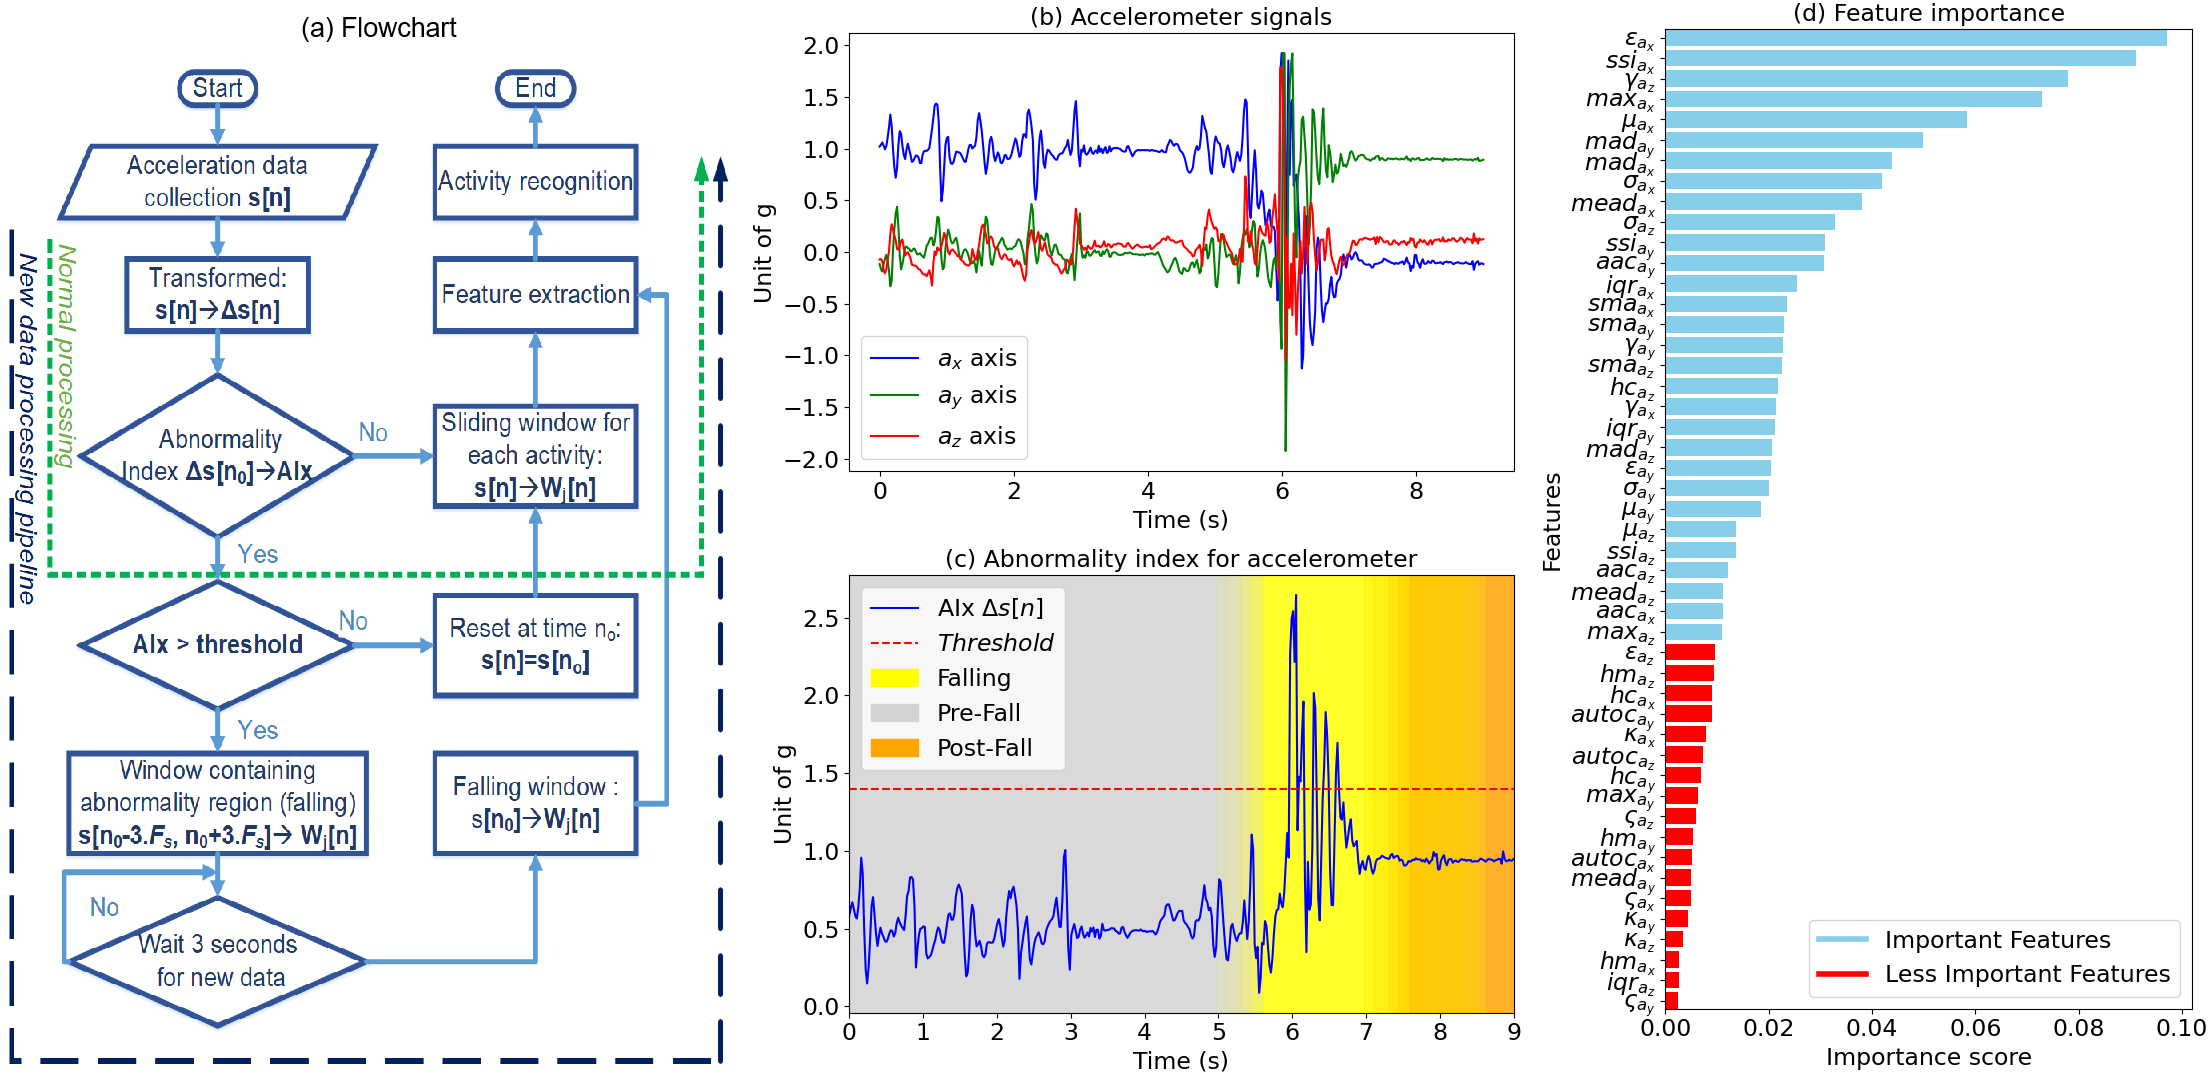
\includegraphics[width=1\linewidth]{Figure/pipeline.png}
    \caption{Sơ đồ pipeline phát hiện bất thường và xử lý dữ liệu: (a) lưu đồ pipeline tổng thể, (b) biến thiên tín hiệu trong hoạt động ngã, (c) kết quả phát hiện bất thường, (d) mức độ quan trọng đặc trưng}
    \label{fig:pipeline}
\end{figure}

\paragraph{Bước 1: Phát hiện chỉ số bất thường}

Chỉ số bất thường ($AIx$) biểu thị sự biến đổi đột ngột trong tín hiệu gia tốc kế tại một thời điểm cụ thể. $AIx$ được tính bằng cách biến đổi tín hiệu $s[n]$ thành chuỗi biến thiên $\Delta s[n]$:

\begin{equation}
\Delta s[n] = \sqrt{\sum_{k \in \{x, y, z\}} \left( a_k[n] - \frac{1}{N} \sum_{n=1}^{N} a_k[n] \right)^2}
\label{eq:delta_s}
\end{equation}

Chỉ số bất thường được xác định khi $\Delta s[n_0]$ vượt ngưỡng $threshold = 1{,}8g$:

\begin{equation}
AIx = \begin{cases}
\Delta s[n_0], & \text{nếu } \Delta s[n_0] > threshold = 1{,}8\,g \\
0, & \text{ngược lại}
\end{cases}
\label{eq:AIx}
\end{equation}

Ngưỡng cửa sổ phát hiện nhỏ $\Delta W = 0{,}5$~giây được chọn dựa trên thời gian tối thiểu của giai đoạn bay trong sự kiện ngã (khoảng 0,34~giây) \cite{Elder_Falling_2019}.

\paragraph{Bước 2: Thu thập dữ liệu xung quanh sự kiện bất thường}

Sau khi phát hiện bất thường tại thời điểm $n_0$, hệ thống thu thập thêm dữ liệu trong vùng:

\begin{equation}
W_j[n], \quad n \in [n_0 - 3 \cdot F_s, \; n_0 + 3 \cdot F_s]
\end{equation}

Cách tiếp cận này tạo ra một cửa sổ dữ liệu chuyên biệt 6 giây xung quanh điểm ngã, tập trung vào vùng tín hiệu quan trọng và cải thiện hiệu suất phát hiện so với cửa sổ trượt cố định.

\paragraph{Bước 3: Phân tích và phân loại}

Dữ liệu trong cửa sổ chuyên biệt này được phân tích để xác định mức độ nghiêm trọng của sự kiện ngã thông qua trích xuất đặc trưng và phân loại. Trong điều kiện bình thường, bước nhảy cửa sổ được đặt bằng kích thước cửa sổ (3~giây) để tiết kiệm năng lượng. Khi $AIx$ vượt ngưỡng, bước nhảy giảm xuống 0,5~giây để tăng tần suất nhận dạng.

\subsubsection{Gán nhãn dữ liệu}

Quy trình gán nhãn gồm ba bước: (1) xác định 11 nhãn tương ứng 11 hoạt động (0 đến 10); (2) phân đoạn và gán nhãn tuần tự theo từng hoạt động; (3) gán nhãn $L_j = k$ cho mỗi cửa sổ $W_j[n]$ thuộc hoạt động $k$. Tất cả hoạt động được quan sát và gán nhãn thủ công bởi hai người giám sát để đảm bảo tính chính xác của dữ liệu.

\subsection{Trích xuất đặc trưng}

\subsubsection{Lựa chọn đặc trưng miền thời gian}

Nghiên cứu ưu tiên các đặc trưng miền thời gian do phù hợp với yêu cầu triển khai trên MCU: không cần biến đổi Fourier tốn kém và có độ phức tạp tính toán thấp. Từ 16 loại đặc trưng ban đầu được xem xét, phương pháp loại trừ dựa trên mức độ quan trọng được áp dụng: giữ lại các đặc trưng có mức độ quan trọng lớn hơn hoặc bằng ngưỡng $0{,}01$ (bằng một nửa độ lệch chuẩn của phân phối mức độ quan trọng, xem Hình~\ref{fig:pipeline}-d).

\subsubsection{Tập đặc trưng tối ưu}

Kết quả lựa chọn cho ra 30 giá trị đặc trưng từ 13 loại đặc trưng. Bảng~\ref{tab:feature} tóm tắt thông tin mô tả các đặc trưng được sử dụng.

\begin{table}[!htb]
    \caption{Các đặc trưng tối ưu được sử dụng trong hệ thống}
    \label{tab:feature}
    \centering
    \footnotesize
    \renewcommand{\arraystretch}{1.5}
    \resizebox{\linewidth}{!}{
    \begin{tabular}{m{0.20\linewidth}m{0.06\linewidth}m{0.38\linewidth}m{0.32\linewidth}}
    \hline\hline
    \rowcolor{gray!20}\textbf{Loại đặc trưng} & \textbf{Trục} & \textbf{Mô tả} & \textbf{Công thức} \\
    \hline\hline
    Năng lượng & x, y & Căn bậc hai của trung bình bình phương tín hiệu &
    $\varepsilon_{a_k} = \sqrt{\frac{1}{M}\sum_{n=1}^{M}a_k^2[n]}$ \\
    Độ lệch tuyệt đối trung bình & x, y, z & Trung bình lệch so với giá trị trung bình &
    $\text{mad}_{a_k} = \frac{1}{M}\sum_{n=1}^{M}|a_k[n]-\mu_{a_k}|$ \\
    Diện tích độ lớn tín hiệu & x, y, z & Tổng giá trị tuyệt đối &
    $\text{sma}_{a_k} = \sum_{n=1}^{M}|a_k[n]|$ \\
    Trung bình & x, y, z & Giá trị trung bình tín hiệu &
    $\mu_{a_k} = \frac{1}{M}\sum_{n=1}^{M}a_k[n]$ \\
    Độ lệch chuẩn & x, y, z & Phân tán tín hiệu quanh giá trị trung bình &
    $\sigma_{a_k} = \sqrt{\frac{1}{M}\sum_{n=1}^{M}(a_k[n]-\mu_{a_k})^2}$ \\
    Tích phân bình phương đơn giản & x, y, z & Tổng bình phương các mẫu &
    $\text{ssi}_{a_k} = \sum_{n=1}^{M}a_k^2[n]$ \\
    Biến đổi biên độ trung bình & x, y, z & Trung bình biến thiên giữa các mẫu liền kề &
    $\text{aac}_{a_k} = \frac{1}{M-1}\sum_{n=1}^{M-1}|a_k[n+1]-a_k[n]|$ \\
    Giá trị lớn nhất & x, z & Cực đại tín hiệu &
    $\text{max}_{a_k} = \max(a_k[n])$ \\
    Độ lệch tuyệt đối trung vị & x, z & Lệch so với giá trị trung vị &
    $\text{mead}_{a_k} = \text{median}(|a_k[n]-\text{median}(a_k)|)$ \\
    Phạm vi tứ phân vị & x, y & Hiệu phần tư 75 và 25 &
    $\text{iqr}_{a_k} = Q_3(a_k[n])-Q_1(a_k[n])$ \\
    Độ phức tạp Hjorth & z & Tỉ lệ linh động của đạo hàm trên linh động tín hiệu &
    $\text{hc}_{a_k} = \text{hm}_{\Delta a_k}/\text{hm}_{a_k}$ \\
    Phạm vi & x, y, z & Hiệu cực đại và cực tiểu &
    $\gamma_{a_k} = \max(a_k[n])-\min(a_k[n])$ \\
    \hline\hline
    \end{tabular}}
\end{table}

\subsection{Tối ưu hóa mô hình Random Forest trên vi điều khiển}

\subsubsection{Bài toán tối ưu hóa siêu tham số}

Giả sử tập dữ liệu $\mathcal{D} = \{(feat_j, L_j)\}_{j=1}^{N_{\Delta t}}$ với nhãn $L_j \in \{1, 2, \ldots, 11\}$. Mô hình RF bao gồm $n\_\text{estimators}$ cây quyết định, mỗi cây có độ sâu tối đa $\text{max\_depth}$. Nhãn dự đoán cuối cùng được xác định bằng bỏ phiếu đa số:

\begin{equation}
\hat{L}_j = \text{Voting}(T_1(feat_j), T_2(feat_j), \ldots, T_{n\_\text{estimators}}(feat_j))
\end{equation}

Giải thuật~\ref{alg:optimization} mô tả quy trình tối ưu hóa siêu tham số, với ràng buộc kích thước mô hình không vượt quá 1~MB và tối đa hóa điểm F1$_{mi}$.

\begin{algorithm}[!htb]
\footnotesize
\caption{\footnotesize Tối ưu hóa siêu tham số cho mô hình ML}
\label{alg:optimization}
\KwIn{Tập dữ liệu $\mathcal{D}$, giới hạn kích thước = 1~MB}
\KwOut{Tham số tối ưu $(n\_estimators^*, max\_depth^*)$ và mô hình RF tương ứng}

Phân chia $\mathcal{D}$ thành $\mathcal{D}_{train}$ (60\%) và $\mathcal{D}_{test}$ (40\%)\;
Khởi tạo $best\_score \leftarrow 0$, $best\_param \leftarrow$ None\;

\For{$max\_depth$ trong $[1, 2, \ldots, 50]$}{
    \For{$n\_estimators$ trong $[1, 2, \ldots, 50]$}{
        Huấn luyện mô hình RF $clf$ trên $\mathcal{D}_{train}$\;
        Đánh giá $clf$ trên $\mathcal{D}_{test}$, tính $score_{val} = F1_{mi}$\;
        \If{$model\_size(clf) < 1$~MB}{
            Xác thực chéo 5-fold trên $\mathcal{D}$ để lấy $score_{cv}$\;
            \If{$|score_{val} - score_{cv}| \leq \varepsilon$ \textbf{và} $score_{val} > best\_score$}{
                $best\_score \leftarrow score_{val}$\;
                $best\_param \leftarrow (n\_estimators, max\_depth)$\;
                $best\_model \leftarrow clf$\;
            }
        }
    }
}
Xuất $best\_model$\;
\end{algorithm}

\subsubsection{Kết quả tối ưu hóa}

Hình~\ref{fig:findparam} trình bày điểm F1$_{mi}$ và kích thước mô hình theo tham số của sáu thuật toán ML được đánh giá. Kết quả cho thấy tham số của mỗi thuật toán phải được ràng buộc thích hợp để đảm bảo kích thước mô hình dưới 1~MB. RF, XGB và LBM đạt F1$_{mi}$ trên 95\% với tham số tối ưu tương ứng.

\begin{figure}[!htb]
    \centering
    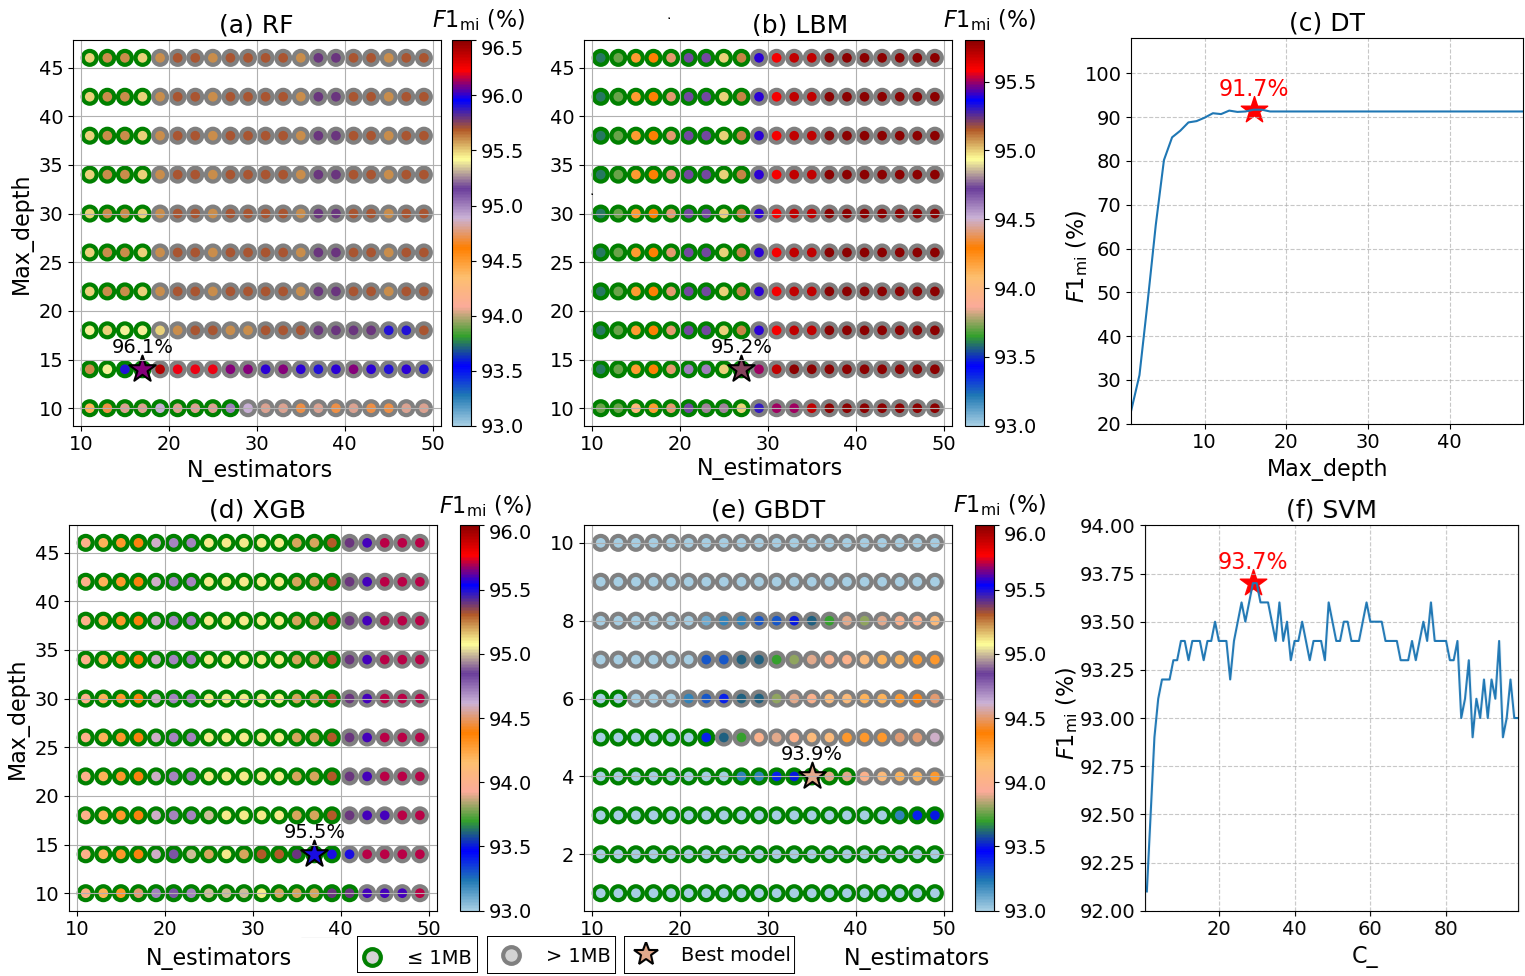
\includegraphics[width=1\linewidth]{Figure/find_parameter.png}
    \caption{Điểm F1$_{mi}$ và kích thước mô hình theo tham số của: (a) RF, (b) LBM, (c) DT, (d) XGB, (e) GBDT, (f) SVM}
    \label{fig:findparam}
\end{figure}

Cấu hình tối ưu của sáu mô hình trên tập dữ liệu riêng được trình bày trong Bảng~\ref{tab:model_config}. Mô hình RF với $n\_\text{estimators} = 17$ và $\text{max\_depth} = 14$ có kích thước 0,9217~MB, thời gian huấn luyện 0,0936~giây và thời gian suy luận 0,0110~giây (tương đương khoảng 3,95~$\mu$s mỗi lần dự đoán).

\begin{table}[!htb]
    \caption{Cấu hình tham số tối ưu các mô hình nhận dạng trên tập dữ liệu riêng}
    \label{tab:model_config}
    \centering
    \footnotesize
    \renewcommand{\arraystretch}{1.2}
    \resizebox{\linewidth}{!}{
    \begin{tabular}{
        >{\arraybackslash}m{0.07\linewidth}
        >{\raggedright\arraybackslash}m{0.28\linewidth}
        >{\centering\arraybackslash}m{0.07\linewidth}
        >{\centering\arraybackslash}m{0.07\linewidth}
        >{\centering\arraybackslash}m{0.07\linewidth}
        >{\centering\arraybackslash}m{0.07\linewidth}
        >{\centering\arraybackslash}m{0.07\linewidth}
        >{\centering\arraybackslash}m{0.07\linewidth}
        >{\centering\arraybackslash}m{0.07\linewidth}
    }
    \hline\hline
    \rowcolor{gray!20}\textbf{Model} & \textbf{Siêu tham số} & $acc$ (\%) & $sen$ (\%) & $spe$ (\%) & $pre$ (\%) & $F1_{mi}$ (\%) & Kích thước (MB) & Trễ (s) \\
    \hline\hline
    RF   & $n{=}17$, $d{=}14$  & 99,3 & 97,0 & 99,6 & 97,1 & \textbf{96,1} & 0,9217 & 0,0110 \\ \hline
    XGB  & $n{=}37$, $d{=}14$  & 99,2 & 96,4 & 99,5 & 96,6 & 95,5 & 0,9398 & 0,0478 \\ \hline
    DT   & $d{=}16$            & 98,5 & 93,3 & 99,1 & 93,6 & 91,7 & 0,0569 & 0,0010 \\ \hline
    GBDT & $n{=}35$, $d{=}4$   & 98,8 & 94,5 & 99,3 & 94,9 & 93,4 & 0,9674 & 0,0149 \\ \hline
    SVM  & $C{=}29$            & 98,9 & 94,8 & 99,4 & 94,6 & 93,7 & 0,2473 & 0,0916 \\ \hline
    LBM  & $n{=}46$, $d{=}22$  & 99,1 & 96,1 & 99,5 & 96,4 & 95,2 & 0,9665 & 0,0080 \\
    \hline\hline
    \end{tabular}}
    \footnotesize \textit{Chú thích: $n$ = số cây; $d$ = độ sâu tối đa; $C$ = tham số điều chuẩn SVM}
\end{table}

\subsubsection{Triển khai TinyML trên vi điều khiển ESP32}

Mô hình RF tối ưu được triển khai trực tiếp trên vi điều khiển ESP32 theo quy trình ba bước:

\textbf{(1) Chuyển đổi và xuất mô hình:} Mô hình đã huấn luyện ($clf$) được chuyển đổi sang mã C thông qua thư viện \texttt{micromlgen}: \texttt{model\_code = port(clf)}, sau đó lưu dưới dạng file header \texttt{random\_forest.h}.

\textbf{(2) Tích hợp mô hình:} File header được nhúng vào firmware vi điều khiển:
\begin{verbatim}
    #include "random_forest.h"
    Eloquent::ml::port::RF rf;
\end{verbatim}

\textbf{(3) Triển khai và thực thi:} Với mỗi vector đặc trưng đầu vào $feat_j$: \texttt{rf.predict(feat\_j)}.

Hình~\ref{fig:suyluan} trình bày thời gian thực tế và thời gian tính toán trên vi điều khiển cho mỗi giai đoạn xử lý. Gia tốc kế lấy mẫu dữ liệu ba trục tại 50~Hz, hệ thống thu thập 150 mẫu trong cửa sổ 3 giây. Sau khi thu thập, trích xuất đặc trưng thực hiện khoảng 8.858~$\mu$s (84.507 dòng lệnh). Mô hình RF với 140.838 dòng lệnh hoàn thành suy luận trong khoảng 733--738~$\mu$s. Tổng độ trễ đầu cuối là xấp xỉ 9.561--9.596~ms.

\begin{figure}[!htb]
    \centering
    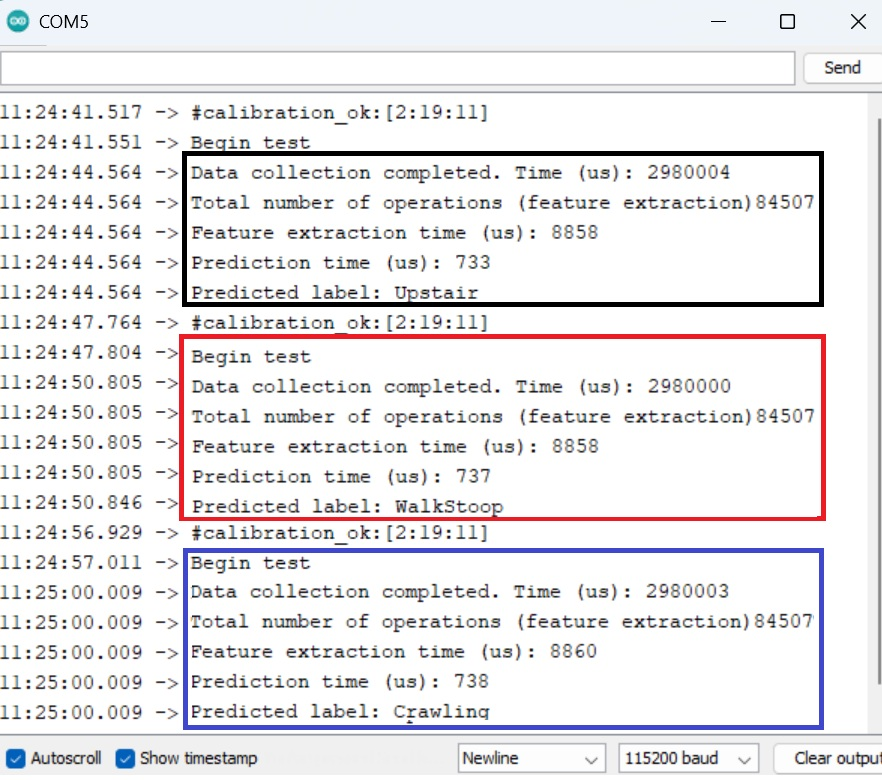
\includegraphics[width=1\linewidth]{Figure/Suyluan.png}
    \caption{Kết quả triển khai dự đoán trên vi điều khiển: thời gian thực tế cho từng giai đoạn xử lý}
    \label{fig:suyluan}
\end{figure}

Mô hình được triển khai là RF gồm 17 cây quyết định, mỗi cây có độ sâu tối đa 14, với kích thước sau biên dịch khoảng 0,92~MB. Độ trễ nhận dạng xấp xỉ 9,561--9,596~ms trên vi điều khiển ESP32, ưu việt hơn một số nghiên cứu liên quan về ứng dụng TinyML trên vi điều khiển \cite{ViManhTuyen2024, Tiny_machine_on_microcontroller, TinyML2023, RIOT_tinyML2025}.